\documentclass[12 pt]{article}         
\usepackage{amsfonts, amssymb}
\usepackage{fancyhdr}
\usepackage{amsmath}
\usepackage{fancyhdr}
\usepackage{verbatimbox}
\usepackage{verbatim}
\usepackage{tikz}
\usetikzlibrary{automata, positioning}
\usepackage{graphicx}

\oddsidemargin=-0.5cm                  
\setlength{\textwidth}{6.5in}          
\addtolength{\voffset}{-20pt}        		
\addtolength{\headsep}{25pt}

\setlength{\headheight}{27.2pt}
\addtolength{\topmargin}{-12.7pt}

\pagestyle{fancy}
\fancyhf{}
\fancyhead[L]{Theory and Practice of Algorithms \\ Homework 6}
\fancyhead[R]{Jingheng Huan \\ \today}
\fancyfoot[C]{\thepage}

\begin{document}

\section*{Problem 1}

(a) True. The dominant term in the polynomial is $2n^3$. As n approaches infinity, the lower-degree terms $(-8n^2 + 32n + 9)$ become negligible in comparison to $2n^3$. Also, we have: $2n^3 - 8n^2 + 32n + 9 \leq C \cdot n^3 \quad$ \text{for some constant } C \text{ and sufficiently large } n.

(b) True. For any real  $p \geq 0$ ,  $n^p$  is a polynomial function, and  $e^n$  is an exponential function. Exponential functions grow faster than any polynomial function. When $n \to \infty$, we have $\lim_{n \to \infty} \frac{n^p}{e^n} = 0$. There exists a constant  $C > 0$  and  $n_0 > 0$  such that for all  $n > n_0$ , we have  $n^p \leq C \cdot e^n$. This implies that  $n^p$  grows slower than  $e^n$.

(c) False. For any real  $p \geq 0$ , as  $n \to \infty$ :
$\lim_{n \to \infty} \frac{e^n}{n^p} = \infty$. This means  $e^n$  grows faster than  $n^p$  and is not bounded above by  $n^p$  multiplied by any constant.

(d) False. The function  $\sqrt{n}$  increases without bound as  $n \to \infty$ , although it grows slower than linear functions. Since  O(1)  represents constant functions that do not grow with  n , and  $\sqrt{n}$  does grow with  n , we have  $\sqrt{n} \notin O(1)$ .

\vspace{1cm}

\section*{Problem 2}
We need to show that there exist positive constants $c_1$, $c_2$, and $n_0$ such that for all $n \geq n_0$: $c_1 n^y \leq (n + x)^y \leq c_2 n^y$. Since x and y are constants and y $>$ 0, we can consider n becomes large.

For the Upper Bound: For $n \geq 1$, we have $(n + x)^y \leq (n + |x|)^y \leq n^y (1 + \frac{|x|}{n})^y$. Using the inequality $(1 + \varepsilon)^y \leq e^{y\varepsilon}$ for $\varepsilon \geq 0$, we get: $(1 + \frac{|x|}{n})^y \leq e^{y \cdot \frac{|x|}{n}} \leq e^{y|x|}$. Thus, we have $(n + x)^y \leq n^y \cdot e^{y|x|} = C_2 n^y$, where $C_2 = e^{y|x|}$ is a constant.

For the Lower Bound: For sufficiently large $n$, we have $(n + x)^y \geq (n - |x|)^y = n^y \left(1 - \frac{|x|}{n}\right)^y$. By using the inequality $(1 - \varepsilon)^y \geq 1 - y\varepsilon$ for $0 < \varepsilon < 1$ and $y > 0$: $\left(1 - \frac{|x|}{n}\right)^y \geq 1 - y \cdot \frac{|x|}{n}$. Therefore, $(n + x)^y \geq n^y \left(1 - \frac{y|x|}{n}\right) \geq n^y \left(1 - \frac{y|x|}{n_0}\right) = C_1 n^y$, for $n \geq n_0$, where $C_1 = 1 - \frac{y|x|}{n_0}$ is positive when $n_0 > y|x|$.

We can say that there exist constants $C_1 > 0$ and $C_2 > 0$ such that: $C_1 n^y \leq (n + x)^y \leq C_2 n^y$, which means that
$(n + x)^y = \Theta(n^y)$.

\vspace{1cm}

\section*{Problem 3}
(a) Applying the Master Theorem for recurrences of the form:

\[
T(n) = a\, T\left( \dfrac{n}{b} \right) + f(n)
\]

We have a = 16, b = 4, f(n) = $n^2$. Then let's compute $\log_b a$:

\[
\log_b a = \log_4 16 = 2
\]
We need to compare f(n) with $n^{\log_b a}$: $f(n) = n^2$ and $n^{\log_b a} = n^{2}$. Since f(n) = $\Theta\left( n^{\log_b a} \right)$, we are in Case 2 of the Master Theorem, then we have:

\[
T(n) = \Theta\left( n^{\log_b a} \cdot \log n \right) = \Theta\left( n^2 \log n \right)
\]

(b) Applying the Master Theorem for recurrences of the form:

\[
T(n) = a\, T\left( \dfrac{n}{b} \right) + f(n)
\]

We have a = 2, b = 4, f(n) = $n^{1/2}$. Then let's compute $\log_b a$:

\[
\log_b a = \log_4 2 = \dfrac{1}{2}
\]

Since $f(n) = \Theta\left( n^{\log_b a} \right)$, we are in Case 2. Then we have $T(n) = \Theta\left( n^{\log_b a} \cdot \log n \right) = \Theta\left( n^{1/2} \log n \right)$.


(c) The recurrence reduces  n  by 2 each time, we expand the recurrence by repeatedly substituting:

\[
T(n) = T(n - 2) + n^2 \\
= T(n - 4) + (n - 2)^2 + n^2 \\
= T(n - 6) + (n - 4)^2 + (n - 2)^2 + n^2 \\
= T(k) + \sum_{i=0}^{t} (n - 2i)^2
\]

k  is a small constant, and  t  is  n/2 . The sum  S  is: $S = \sum_{i=0}^{t} (n - 2i)^2$

This sum consists of approximately  n/2  terms of decreasing squares starting from  $n^2$  down to a constant. The sum of squares of the first  m  positive integers is  $\sum_{k=1}^{m} k^2 = \frac{m(m + 1)(2m + 1)}{6}$. However, our sum is similar to summing squares from  n  down to a small number. To estimate  S , we can consider it proportional to  $n^3$ : $S \approx \int_{0}^{n/2} (n - 2x)^2 \, dx$. Then let's compute the integral:

\[
S \approx \int_{0}^{n/2} (n - 2x)^2 \, dx \\
= \left[ (n - 2x)^3 / (-6) \right]_0^{n/2} \\
= \left( 0 - \frac{n^3}{6} \right) = \frac{n^3}{6}
\]

The total sum  S  is proportional to  $n^3$ , so: $T(n) = T(k) + S = \Theta(n^3)$

(d) Applying the Master Theorem for recurrences of the form:

\[
T(n) = a\, T\left( \dfrac{n}{b} \right) + f(n)
\]

we have a = 3, bj = 3, \( f(n) = \dfrac{n}{\log n} \), we calculate $\log_b a = \log_3 3 = 1$. So $n^{\log_b a} = n$.

Then let's compare  f(n)  with  $n^{\log_b a}$ : \( f(n) = \dfrac{n}{\log n} = \dfrac{n^{\log_b a}}{\log n} \)
f(n)  is slightly smaller than  n  due to the  $\log n$  denominator. Determine which case of the Master Theorem applies:
The Master Theorem doesn’t directly handle  f(n)  being smaller than  $n^{\log_b a}$  by a logarithmic factor. Since \( f(n) = \dfrac{n}{\log n} = n^{\log_b a} / \log n = o\left( n^{\log_b a} \right) \), but not polynomially smaller. The recurrence resembles \( T(n) = 3\, T\left( \dfrac{n}{3} \right) + n \), which has a solution  $T(n) = \Theta(n \log n)$. Because  f(n)  is \( \dfrac{n}{\log n} \), which is  n  divided by  $\log n$ , the overall  T(n)  will be $\Theta(n \log \log n)$.

\section*{Problem 4}
Pseudocodes are also written in matrixmult.py files as code comments.

\subsection*{Pseudocode and runtime analysis}
\begin{verbatim}
function matrix_mul(A, B):
    m = number of rows in A
    k = number of columns in A (also number of rows in B)
    n = number of columns in B
    Initialize C as an m x n matrix filled with zeros
    for i from 0 to m - 1:
        for j from 0 to n - 1:
            sum = 0
            for l from 0 to k - 1:
                sum = sum + A[i][l] * B[l][j]
            C[i][j] = sum
    return C
\end{verbatim}

\begin{verbatim}
function matrix_mul(A, B):
Executed: Once when the function is called.
Time Complexity: O(1)
\end{verbatim}

\begin{verbatim}
m = number of rows in A
Executed: Each line is executed once.
Time Complexity: O(1) per line.
Total Time: O(1)
\end{verbatim}

\begin{verbatim}
k = number of columns in A (also number of rows in B)
Executed: Each line is executed once.
Time Complexity: O(1) per line.
Total Time: O(1)
\end{verbatim}

\begin{verbatim}
n = number of columns in B
Executed: Each line is executed once.
Time Complexity: O(1) per line.
Total Time: O(1)
\end{verbatim}

\begin{verbatim}
Initialize C as an m x n matrix filled with zeros
Executed: Once.
Operations: Initializes an  m * n  matrix.
Time Complexity: O( m * n )
The outer list comprehension runs  m  times.
The inner list comprehension runs  n  times for each outer iteration.
Total Time: O( m * n )
\end{verbatim}

\begin{verbatim}
for i from 0 to m - 1:
Executed:  m  times.
Time Complexity: Loop overhead is negligible; loop body determines total time.
\end{verbatim}

\begin{verbatim}
for j from 0 to n - 1:
Executed:  m * n  times (nested inside the i loop).
Time Complexity: Loop overhead is negligible.
\end{verbatim}

\begin{verbatim}
sum = 0
Executed:  m * n  times
Time Complexity: O(1) per execution.
Total Time: O( m * n )
\end{verbatim}

\begin{verbatim}
for l from 0 to k - 1:
Executed:  m * n  times
Iterations per Execution:  k  times.
Time Complexity: Loop overhead is negligible
\end{verbatim}

\begin{verbatim}
sum = sum + A[i][l] * B[l][j]
Executed:  m * n * k  times
Time Complexity per Execution: O(1)
Total Time: O( m * n * k )
\end{verbatim}

\begin{verbatim}
C[i][j] = sum
Executed:  m * n  times
Time Complexity per Execution: O(1)
Total Time: O( m * n )
\end{verbatim}

\begin{verbatim}
return C
Executed: Once.
Time Complexity: O(1)
\end{verbatim}

Overall runtime is $O(m\times n \times k)$

\subsection* {Theoretical Runtime for Each Matrix Shape}

Many Rows x Few Columns
Matrix  A :  m = N ,  k = 4. Matrix  B :  k = 4 , \( n = \dfrac{N}{4} \)

Total Time Complexity:
\[
O(m \times n \times k) = O\left( N \times \dfrac{N}{4} \times 4 \right) = O(N^2)
\]

Square Matrices
Matrix  A :  m = N ,  k = N. Matrix  B :  k = N ,  n = N 

Total Time Complexity:
\[
O(m \times n \times k) = O(N \times N \times N) = O(N^3)
\]

Few Rows x Many Columns
Matrix  A : \( m = \dfrac{N}{4} \),  k = N. Matrix  B :  k = N ,  n = 4N 
Total Time Complexity:
\[
O(m \times n \times k) = O\left( \dfrac{N}{4} \times 4N \times N \right) = O(N^3)
\]

\begin{table}[h!]
\centering
\begin{tabular}{|c|c|c|c|}
\hline
$N$ & Many Rows x Few Columns (ms) & Square Matrices (ms) & Few Rows x Many Columns (ms) \\
\hline
4   & 0.009 & 0.010 & 0.007 \\
\hline
8   & 0.008 & 0.039 & 0.031 \\
\hline
16  & 0.025 & 0.215 & 0.201 \\
\hline
32  & 0.108 & 1.493 & 1.485 \\
\hline
64  & 0.314 & 11.147 & 10.583 \\
\hline
128 & 1.025 & 67.544 & 61.873 \\
\hline
256 & 3.331 & 511.097 & 521.692 \\
\hline
512 & 13.584 & 4585.500 & 4909.575 \\
\hline
\end{tabular}
\caption{Measured average runtimes of 5 runs for different matrix sizes and shapes}
\label{tab:runtime_data}
\end{table}

Units: Time is measured in milliseconds (ms).

\begin{figure}[h]
    \centering
    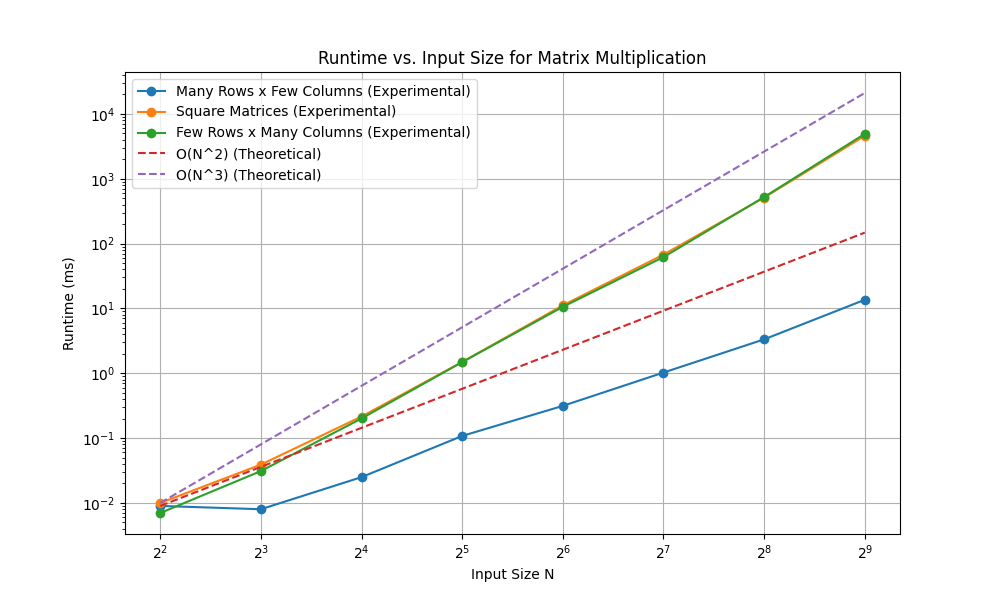
\includegraphics[width=0.5\textwidth]{HW6/Q4.png}
    \caption{The plot of the relationship between runtime and the input size N. Here I also take log on both x-axis and y-axis.}
    \label{fig:my_image}
\end{figure}


\subsection*{Analysis of Results}

\subsubsection*{1. Many Rows x Few Columns (Expected $O(N^2)$)}
The runtime increases approximately with $N^2$. When $N$ doubles, the runtime nearly quadruples.
    \begin{itemize}
        \item $N = 32$ to $N = 64$: Runtime increases from 0.108 ms to 0.314 ms (about 2.9 times).
        \item $N = 64$ to $N = 128$: Runtime increases from 0.314 ms to 1.025 ms (about 3.26 times).
        \item $N = 128$ to $N = 256$: Runtime increases from 1.025 ms to 3.331 ms (about 3.25 times).
    \end{itemize}
These results suggest quadratic growth, consistent with $O(N^2)$.


\subsubsection*{2. Square Matrices (Expected $O(N^3)$)}
Runtime increases significantly as $N$ increases. When $N$ doubles, runtime approximately multiplies by 8.
    \begin{itemize}
        \item $N = 32$ to $N = 64$: Runtime increases from 1.493 ms to 11.147 ms (about 7.47 times).
        \item $N = 64$ to $N = 128$: Runtime increases from 11.147 ms to 67.544 ms (about 6.06 times).
        \item $N = 128$ to $N = 256$: Runtime increases from 67.544 ms to 511.097 ms (about 7.57 times).
        \item $N = 256$ to $N = 512$: Runtime increases from 511.097 ms to 4585.500 ms (about 8.97 times).
    \end{itemize}
Results suggest cubic growth, consistent with $O(N^3)$.

\subsubsection*{3. Few Rows x Many Columns (Expected $O(N^3)$)}
Runtime growth is similar to square matrices. When $N$ doubles, runtime increases by approximately 8 times.

    \begin{itemize}
        \item $N = 32$ to $N = 64$: Runtime increases from 1.485 ms to 10.583 ms (about 7.12 times).
        \item $N = 64$ to $N = 128$: Runtime increases from 10.583 ms to 61.873 ms (about 5.85 times).
        \item $N = 128$ to $N = 256$: Runtime increases from 61.873 ms to 521.692 ms (about 8.43 times).
        \item $N = 256$ to $N = 512$: Runtime increases from 521.692 ms to 4909.575 ms (about 9.41 times).
    \end{itemize}
Results suggest cubic growth, consistent with $O(N^3)$.


\subsection*{Comparison of Theory and Practice}
The potential reasons of divergence between theory and practice:
    \begin{itemize}
        \item Python interpreter overhead.
        \item System load and background processes.
        \item Memory caching effects.
        \item Memory access order impacts caching efficiency.
    \end{itemize}

\vspace{1cm}

\section*{Problem 5}

\begin{verbatim}
function matching_length_sub_strs(s, c1, c2):
Initialize c1_ranges as result of find_ranges(c1)
Initialize c2_ranges as result of find_ranges(c2)
Initialize result as an empty set

for each length in c1_ranges:
    if length exists in c2_ranges:
        c1_starts = c1_ranges[length]
        c2_starts = c2_ranges[length]
        for each c1_start in c1_starts:
            for each c2_start in c2_starts:
                Add (c1_start, c2_start, length) to result

return result

function find_ranges(char):
Initialize ranges as an empty dictionary with lists as default values
Initialize i as 0
Initialize n as length of s
while i < n:
if s[i] == char:
start = i
while i < n and s[i] == char:
Increment i by 1
length = i - start
Add start to ranges[length]
else:
Increment i by 1
return ranges
\end{verbatim}


\begin{verbatim}
function matching_length_sub_strs(s, c1, c2):
Executed: Once when the function is called.
Time Complexity: O(1)
\end{verbatim}

\begin{verbatim}
Initialize c1_ranges as result of find_ranges(c1)
Executed: Once (calls find_ranges function).
Time Complexity: O(n) since find_ranges iterates through string s.
\end{verbatim}

\begin{verbatim}
Initialize c2_ranges as result of find_ranges(c2)
Executed: Once (calls find_ranges function).
Time Complexity: O(n) since find_ranges iterates through string s.
\end{verbatim}

\begin{verbatim}
Initialize result as an empty set
Executed: Once.
Time Complexity: O(1)
\end{verbatim}

\begin{verbatim}
for each length in c1_ranges:
Executed: L1 times, where L1 is the unique lengths in c1_ranges.
Time Complexity: O(L1)
\end{verbatim}

\begin{verbatim}
if length exists in c2_ranges:
Executed: L1 times, checking existence in c2_ranges.
Time Complexity: O(1) per check
Total Time: O(L1)
\end{verbatim}

\begin{verbatim}
c1_starts = c1_ranges[length]
Executed: L1 times, assigning list from dictionary.
Time Complexity: O(1) per assignment
Total Time: O(L1)
\end{verbatim}

\begin{verbatim}
c2_starts = c2_ranges[length]
Executed: L1 times, assigning list from dictionary.
Time Complexity: O(1) per assignment
Total Time: O(L1)
\end{verbatim}

\begin{verbatim}
for each c1_start in c1_starts:
Executed: L1 * N1 times, where N1 is average starts per length in c1_ranges.
Time Complexity: Loop overhead is negligible; body determines total time.
\end{verbatim}

\begin{verbatim}
for each c2_start in c2_starts:
Executed: L1 * N1 * N2 times, where N2 is average starts per length in c2_ranges.
Time Complexity: Loop overhead is negligible.
\end{verbatim}

\begin{verbatim}
Add (c1_start, c2_start, length) to result
Executed: L1 * N1 * N2 times, adding to result set.
Time Complexity per Execution: O(1)
Total Time: O(L1 * N1 * N2)
\end{verbatim}

\begin{verbatim}
return result
Executed: Once.
Time Complexity: O(1)
\end{verbatim}

\begin{verbatim}
function find_ranges(char):
Executed: Once per call.
Time Complexity: O(1)
\end{verbatim}

\begin{verbatim}
Initialize ranges as an empty dictionary
Executed: Once.
Time Complexity: O(1)
\end{verbatim}

\begin{verbatim}
Initialize i as 0
Executed: Once.
Time Complexity: O(1)
\end{verbatim}

\begin{verbatim}
Initialize n as length of s
Executed: Once.
Time Complexity: O(1)
\end{verbatim}

\begin{verbatim}
while i < n:
Executed: n times, iterates through each character in s.
Time Complexity: O(n)
\end{verbatim}

\begin{verbatim}
if s[i] == char:
Executed: Up to n times, depending on occurrences of char in s.
Time Complexity: O(1) per check
Total Time: O(n)
\end{verbatim}

\begin{verbatim}
start = i
Executed: O(1) per match, up to n times.
Time Complexity: O(n)
\end{verbatim}

\begin{verbatim}
while i < n and s[i] == char:
Executed: Up to n times (increments until char changes).
Time Complexity: O(n)
\end{verbatim}

\begin{verbatim}
Increment i by 1
Executed: n times across matches.
Time Complexity: O(n)
\end{verbatim}

\begin{verbatim}
length = i - start
Executed: O(1) per match.
Time Complexity: O(n)
\end{verbatim}

\begin{verbatim}
Add start to ranges[length]
Executed: O(1) per match, up to n times.
Time Complexity: O(n)
\end{verbatim}

\begin{verbatim}
return ranges
Executed: Once.
Time Complexity: O(1)
\end{verbatim}

The overall runtime of $matching_length_sub_strs$ is $O(n + L_1 \times N_1 \times N_2)$

In the worst case, this is $O(n^3)$.

\begin{table}[h!]
\centering
\begin{tabular}{|c|c|c|c|}
\hline
$N$ & Best Case Time (ms) & Worst Case Time (ms) & Random Input Time (ms) \\
\hline
512   & 0.051    & 7.216      & 2.209     \\
\hline
1024  & 0.209    & 34.161     & 14.929    \\
\hline
2048  & 0.773    & 143.085    & 57.414    \\
\hline
4096  & 3.292    & 757.593    & 244.013   \\
\hline
8192  & 17.775   & 4126.838   & 1338.515  \\
\hline
16384 & 74.511   & 790339.969 & ---       \\
\hline
\end{tabular}
\caption{Measured average runtimes of 5 runs for different input sizes and cases}
\label{tab:runtime_data}
\end{table}



\noindent\textbf{Collaborators: None}

\end{document}